\documentclass[english]{extarticle}
\usepackage{setspace}
\usepackage{titling}
\usepackage[sfdefault]{roboto}
\usepackage[T1]{fontenc}
\usepackage[latin9]{inputenc}
\usepackage[top=1.5cm, bottom=2cm, left=2cm, right=2cm]{geometry}
\usepackage{fancyhdr}
\usepackage{graphicx}
\usepackage{hyperref}
\usepackage[usenames, dvipsnames]{color}
\usepackage{babel}
\fancypagestyle{plain}

\pagestyle{fancy}
\renewcommand{\headrulewidth}{0pt}
\renewcommand{\footrulewidth}{0.6pt}

\hypersetup{
    colorlinks,
    citecolor=black,
    filecolor=black,
    linkcolor=black,
    urlcolor=[rgb]{0, 0, 0.6}
}

\setlength{\droptitle}{-50pt}

\definecolor{primary}{RGB}{80, 80, 80}
\definecolor{secondary}{RGB}{140, 0, 0}
\definecolor{tertiary}{RGB}{120, 0, 0}
\definecolor{light}{RGB}{180, 180, 180}

\newcommand{\mySect}[2]{
    \section*{\textcolor{secondary}{#1}\hfill{\footnotesize\textmd{{#2}}}}
    \vspace{-2em}
    \textcolor{tertiary}{\hrule}
    \vspace{0.5em}
}

% \lfoot{\parbox{3.7cm}{
\includegraphics{phone} +818077993837}}
\lfoot{
\includegraphics{mail} \href{mailto:markhedleyjones@gmail.com}{markhedleyjones@gmail.com}}
% \cfoot{\hspace{-1.2cm}
\includegraphics{mail} \href{mailto:markhedleyjones@gmail.com}{markhedleyjones@gmail.com}}
\rfoot{\href{http://markhedleyjones.com}{markhedleyjones.com}}

\fontfamily{phv}
\begin{document}

{
    \noindent
    \centering
    \Huge\bfseries \textcolor{primary}{MARK HEDLEY JONES}\\
}
\vspace{3mm}
\textcolor{light}{\hrule}
\vspace{3mm}
\noindent
\begin{minipage}[h]{0.78\textwidth}

    \begin{center}
    \begin{minipage}[t]{1.0\textwidth}
    \large
    Experience in both research and commercial development environments\\
    Robotic system design, implementation, and development\\
    Holds doctoral, masters and bachelor degrees\\
    \end{minipage}
    \end{center}


    % \textcolor{light}{\hrule}
    \vspace{5mm}

    \noindent\begin{center}\parbox[l]{8cm}{
    {Nationalities:\hfill{\textmd{\small New Zealand}} \& {\textmd{\small British}}}{}\\
    {Date of birth:\hfill{\textmd{\small October 1984}}}{}\\
    {Languages:\hfill{\textmd{\small English (Native), Japanese (N3)}}}
    }\end{center}

\end{minipage}
\noindent
% \hspace{2mm}
\begin{minipage}[h]{0.18\textwidth}
\vspace{5mm}
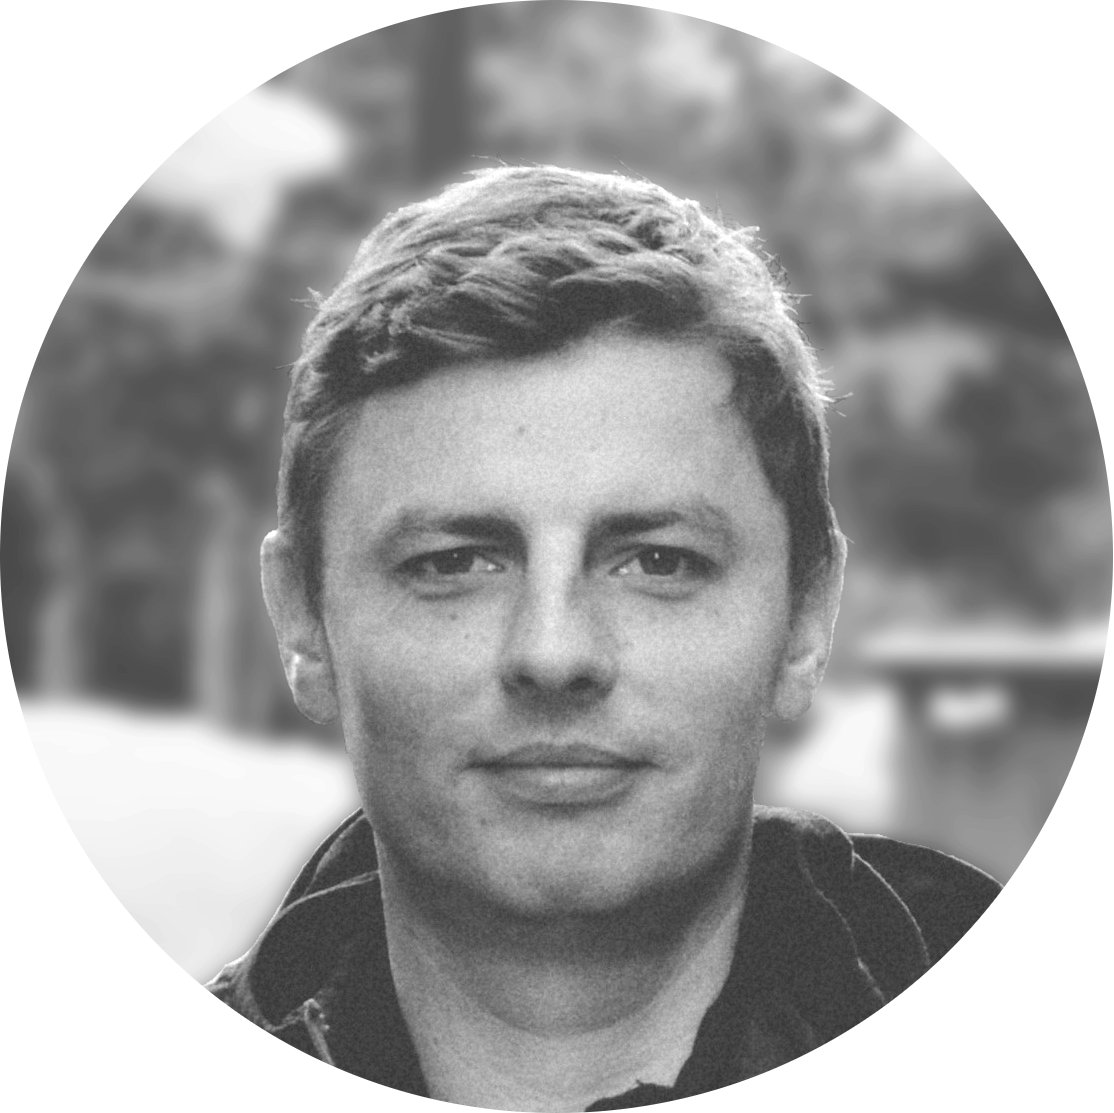
\includegraphics[width=1.2\textwidth]{Profile.png}
\end{minipage}

\mySect{SKILLS}{}

\subsection*{Technical:}
\begin{itemize}
    \item {Experience developing \textbf{ROS} based robotic systems across four multi-million dollar projects (7+ years)}
    \item {Implementation of computer vision systems (\textbf{OpenCV} \& \textbf{Deep Learning}) for real-time identification}
    \item {Designing mechanical components and modeling using CAD tools (\textbf{SolidWorks}, 6+ years)}
    \item {Software development in \textbf{Linux} (10+ years) with \textbf{C/C++}(7+ years), and \textbf{Python} (7+ years)}
    \item {Electronic design (PCB/embedded) and including fail-safe system architecture}
\end{itemize}

\subsection*{Communication:}
\begin{itemize}
    \item {Managing a small research team (6-10 people) and presenting progress at board meetings}
    \item {Publishing research papers, presenting at international conferences, and writing theses}
    \item {Mentoring post-graduate students and demonstrating in undergraduate laboratories}
\end{itemize}

\subsection*{Miscellaneous:}
\begin{itemize}
    \item {Financial management of project spending with direct control of company credit cards}
    \item {Workshop competency including use of mills (manual \& CNC), lathes, MIG welder}
    % \item {Can drive in Japan and New Zealand (with licences)}
\end{itemize}
\mySect{EMPLOYMENT}{}

\subsection*{Software Engineer - Mapping \& Simulation \& Object Detection \\\textmd{\footnotesize Based at \href{https://www.seqsense.com/}{SEQSENSE} \hfill{} \textbf{November 2018 -- Present}}}
Software engineering focusing on map creation, simulation environments, and object detection
Developing and maintaining a 3D map generation system that runs across desktop, cloud, and our robot (real-time).
\\Tasks include:
\begin{itemize}
    \item creation of an on-line lidar-based mapping system to generate point-cloud-data (PCD) maps;
    \item development of an on-line object detection system based on lidar and camera inputs;
    \item developing and maintaining a simulation environment (\textbf{Gazebo}) that closely mimics robot behaviour;
    \item producing and maintaining accurate robot model definitions (\textbf{URDF}) from CAD models.
\end{itemize}

\subsection*{Post-Doctoral Researcher - Autonomous Navigation\\\textmd{\footnotesize Based at \href{https://www.roboticsplus.co.nz/}{Robotics Plus Ltd.}, employed by \href{https://auckland.ac.nz}{The University of Auckland} \hfill{} \textbf{December 2017 -- October 2018}}}
Developed navigation software for heavy-duty vehicles used in outdoor environments.
\\Tasks included:
\begin{itemize}
    \item integrating and tuning real-time \textbf{SLAM}, point-cloud processing, and path-planning in orchards;
    \item selecting and integrating lidar, cameras, radars, compasses, encoders, IMUs, and GNSS systems;
    \item personally responsible for the safety of people and infrastructure regarding our autonomous vehicle;
    \item development of a web-based graphical user interface to monitor and control our autonomous vehicle.
\end{itemize}

\subsection*{Post-Doctoral Researcher - Robotic Hardware Development \\\textmd{\footnotesize \href{https://www.roboticsplus.co.nz/}{Robotics Plus Ltd.}, employed by \href{https://waikato.ac.nz}{The University of Waikato} \hfill{} \textbf{March 2015 -- December 2017}}}
Designed and built a heavy-duty outdoor vehicle, fruit harvesting robot, pollination robot.\\
Designed robotic systems (hardware \& firmware) and managed a team of post-graduate researchers.\\
Tasks included:
\begin{itemize}
    \item financial management, ordering, report writing, project planning, and resource coordination;
    \item component selection, vehicle design and assembly, electrical hardware integration and testing.
    \item managing a research team consisting of doctoral and masters students, coordinating between universities;
    \item developing \textbf{ROS} based systems to control robotic arms, precision spraying systems, and an electric vehicle;
\end{itemize}

\subsection*{Previously:}

\subsubsection*{Web Developer \textmd{\footnotesize Department of Science \& Engineering (The University of Waikato) \hfill{} \textbf{2013 -- 2014}}}
\vspace{-2mm}
Developed an interactive tutorial web-app used by all 1st year electronic engineering students. (\href{https://markhedleyjones.com/projects/electronics-tutorial-website}{More})

\subsubsection*{Lab Demonstrator \textmd{\footnotesize Department of Science \& Engineering (The University of Waikato) \hfill{} \textbf{2013 -- 2014}}}
\vspace{-2mm}
Managed electronics laboratories, demonstrated electronic concepts, and graded assignments and final exams.

\subsubsection*{Web Developer \textmd{\footnotesize Self-employed \hfill{} \textbf{2010 -- 2013}}}
\vspace{-2mm}
Built an online rental-property advertising company. Sourced investment, developed partnerships, marketing. (\href{https://markhedleyjones.com/projects/houser}{More})

\subsubsection*{Researcher \textmd{\footnotesize Department of Biological Science (The University of Waikato) \hfill{} \textbf{2010}}}
\vspace{-2mm}
Created electric field simulations of an electro-fishing boat to improve its ability to catch pest fish species. (\href{https://researchcommons.waikato.ac.nz/bitstream/handle/10289/11289/Use%20of%20Electrofishing.pdf}{More})

\subsubsection*{Audio/Visual installation \textmd{\footnotesize 021SOUNDTECH \hfill{} \textbf{2006 -- 2007}}}
\vspace{-2mm}
Traveled across New Zealand installing high-end audio equipment into under-construction public venues.

\subsubsection*{Assembly Technician \textmd{\footnotesize \href{https://rennacs.com/}{RENNACS} \hfill{} \textbf{2005 -- 2006}}}
\vspace{-2mm}
Assembled, soldered, flashed, tested, and debugged automotive fault-code readers.

\subsubsection*{Further back:}
Owner/operator of a property-maintenance business;
owner/operator of a rental-property advertising website;
farm-hand;
house restoration;
photo printing in a film processing lab;
customer service at a delicatessen;
cooking pizzas at a fast-food resturant;
swimming pool maintenance and sample gathering;
photo-cataloging high-voltage electrical substation equipment;
painting tapestry canvases;
computer assembly, repairs \& maintenance.
\mySect{EDUCATION}{}

\begin{itemize}

    \item \textbf{Doctorate of Philosophy} -- The Electrical Properties of Interfacial Double Layers\textbf{\footnotesize\hfill 2011 -- 2015}\begin{itemize}
        \item Modelled electrical conductivity of implanted medical electrodes using circuit simulation tools
        \item Conducted automated electrical impedance measurements \emph{in a hospital operating theatre}
        \item Developed software libraries to automate oscilloscopes and function generators
    \end{itemize}
    \item \textbf{Masters of Engineering} with First Class Honours\textbf{\footnotesize\hfill 2009}
    \begin{itemize}
        \item Simulated a novel design of high-frequency power sensor (170\,GHz) to determine performance
        \item Built and measured the performance of scale models of RF sensors to verify simulation results
        \item Visited NIST, Boulder Colorado, to find understand sensor traceability testing at the US national level
    \end{itemize}
    \item \textbf{Bachelor of Science} -- Major in Electronics focusing on Mechatronics\textbf{\footnotesize\hfill 2005 -- 2008}
\end{itemize}


\vspace{1.0cm}

\mySect{AWARDS \& SCHOLARSHIPS}{}
\begin{tabular}{lrr}
$\bullet$ Waikato Doctoral Scholarship & \$ 56 000 USD & 2010 \\
$\bullet$ Agilent Technologies Research Scholarship & \$ 36 000 USD & 2009 \\
$\bullet$ Summer Research Scholarship & \$ 5 000 USD & 2008 \\
$\bullet$ ENZcon -- best research paper & & 2011 \\
$\bullet$ ENZcon -- runner up best presentation \hspace{6.1cm} & & \hspace{0.7cm} 2014 \\
\end{tabular}

\vspace{1.0cm}

\mySect{LICENCES / VISAS}{}
\begin{tabular}{l}
$\bullet$ Japanese Permanent Residency \\
$\bullet$ Japanese Drivers Licence \\
$\bullet$ New Zealand Drivers License \\
\end{tabular}

\vspace{1.0cm}

\mySect{PHILOSOPHY}{}
\begin{centering}
\onehalfspacing
\noindent
The ability to teach yourself is more valuable than your education\\
\noindent
Test ideas early and invest time in reducing the cost to re-test\\
\noindent
Something isn't right just because other people are doing it\\
\end{centering}

\vspace{1.0cm}

\mySect{PUBLICATIONS}{}
\noindent
Please see \href{https://markhedleyjones.com/about}{my website} for an up-to-date list of publications.

\vspace{1.0cm}

\mySect{REFEREES}{}
\noindent
Available upon request


\end{document}
